This section will provide information about how the web application is implemented. First the different frameworks that was used during development are listed and then the conducted tests are presented. 

\subsubsection{Frameworks}
\label{sec:web_frame}
The frameworks was used to ease implementing the system. The following frameworks are integrated in the system and the system is built on them. To read more about the frameworks, see the References page.

\paragraph{Backbone}
Backbone\cite{web_1} is a light-weight framework that loosely follows the \textbf{MVC} (model, view, controller) pattern. Out of the \textbf{MVC} components, backbone only has models and views, and the view behaves much like a view and a controller. \textbf{Models} are the parts of code that retrieves and populates data (for example, the model Experiment will obtain and populate the experiments resulting from a search). \textbf{Views} are the HTML representation of models, and they change as models change (When the Experiment model is populated, it is immediately presented on the view that contains that Experiment).
Backbone makes use of \textbf{Events}, where other objects can trigger events and listen to them, which is an effective way to promote decoupling between components. It also uses \textbf{Collections}, that are ordered sets of models. A collection will automatically be provided with underscore array and collection methods for convenient set manipulations (You can, for example loop through a collection with .each() instead of writing a for-loop). We chose to use backbone because we wanted more structure in our web application. With more structure, it is easier to collaborate as we can divide up the work - keeping our javascript in various model, collection and view files.

\paragraph{Bootstrap}
Bootstrap\cite{web_2} is a front-end framework that contains HTML and CSS-based design templates for typography, buttons, forms, navigations, and the like. Instead of creating our own buttons, deciding on colors, how big they are, and micromanaging how they fit with everything else on the page, we can use bootstraps templates that handles all of that for us, leaving us able to focus on architecture. We chose to use it to save time on development and make the look of our web app easily customizable.

\paragraph{AJAX}
AJAX\cite{web_3} stands for \textbf{Asynchronous Javascript and XML}. It is a technique for creating fast and dynamic web pages. Despite the name, the use of XML is not required; JSON is often used instead, as we have done in our web app. AJAX allows web pages to be updated asynchronously by exchanging small amounts of data with the server, so that you only update parts of a webpage without having to reload the entire page (like websites that don’t use AJAX has to). For example, when “search” is clicked in our navigation bar, only the bottom half of the website is being updated, and displaying the search view. The navigation bar does not have to be reloaded, but remains as is on top.

\paragraph{JSON}
JSON\cite{web_4} is short for \textbf{javaScript Object Notation} and is a format that is primary used to transmit data between a server and web application instead of using XML or other formats.
JSON is formatted as text which is easy to read consisting of attribute-value pairs.
JSON was used in this application because JSON uses the same syntax as JavaScript and therefore we do not need to make our own parser as we would have to do for e.g. XML. JSON does also work very well together with Backbone as it has integrated methods using the JSON format.

\paragraph{RequireJS}
RequireJS\cite{web_5} is a file and module loader for JavaScript. RequireJS lets files require other files much like \texttt{\#include} in java this is very handy for the programmer. It is used because it helps to structure the application.

\paragraph{JQuery}
The purpose of JQuery\cite{web_6} is to make it easier to use Javascript on a website. It takes a lot of common tasks that require many lines of javascript code to accomplish, and wraps them into methods that you can call with a single line of code. It simplifies other things as well, like AJAX calls and DOM manipulation, both of which are in frequent use in our web application.

\subsubsection{Testing frameworks}
For testing we have used three libraries to make testing easier: chai, mocha and sinon. Together they let us make a page for testing where all tests and results will be shown visually.
These libraries or testing frameworks will be discussed below.

\paragraph{Chai \& Mocha}
Mocha\cite{web_8} is a test framework while Chai\cite{web_7} is an expectation framework. While Mocha setups and describes test suites, Chai provides convenient helpers to perform all kinds of assertions against javascript code. We use these frameworks to do unit testing on our models and collections.

\paragraph{Sinon}
Sinon\cite{web_9} is a framework used to \textit{“fake environment”}. When doing unit testing, we don’t want to depend on things that are external to the unit of code that we are testing. We can use Sinon for stubbing and mocking external dependencies and to keep control on side effects against them. For example, we can use Sinon to create spies to see if an event has been triggered, and to create fake servers that respond with fake preplanned responses to our queries.

\subsubsection{Our Tests}
We have performed unit tests on our model and collection files, all of which can be found in our root folder under \filePath{/tests/}, more specifically: \filePath{genomizer-web \slash tests\slash}. To see the tests, simply open the index.html in a web browser, and they will run.
%FIGURE X

\begin{figure}[h]
\centering
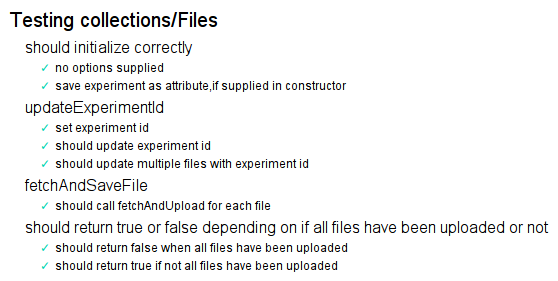
\includegraphics[width=1\textwidth]{web_test_collectionFiles.png}
\caption{The tests for the Files collection, all of which it has passed.}
\label{fig:web_test_collectionFiles}
\end{figure}

\refer{fig:web_test_collectionFiles} displays our tests of the \textit{Files} collection, checking that the collection initializes correctly, that it can update an experiment’s ID, that it can fetch and save a file, that it can check if a file has been uploaded or not.
%FIGURE X1
\begin{figure}[h]
\centering
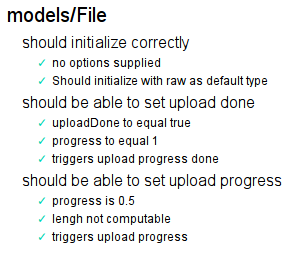
\includegraphics[width=0.6\textwidth]{web_test_modelsFile.png}
\caption{The tests for the File model, all of which it has passed.}
\label{fig:web_test_modelsFile}
\end{figure}

\refer{fig:web_test_modelsFile} displays our tests of the \textit{File} model, checking that the model initializes correctly, that it can set itself to be fully uploaded, and that it can set itself to have an upload progress (for example, a file that is halfway uploaded should set it’s progress to 0.5).
%FIGURE X2
\begin{figure}[h]
\centering
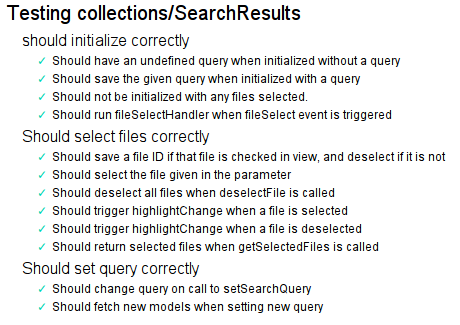
\includegraphics[width=1\textwidth]{web_test_collectionsSearchResults.png}
\caption{The tests for the SearchResults collection, all of which it has passed.}
\label{fig:web_test_collectionsSearchResults}
\end{figure}

\refer{fig:web_test_collectionsSearchResults} displays our tests of the SearchResults collection, checking that the collection initializes correctly, that it can select files correctly, that it can set a new query and that it will fetch new models upon getting a new query.
%FIGURE X3
\begin{figure}[h]
\centering

\includegraphics[width=0.6\textwidth]{web_test_modalAC.png}
\caption{The test for the ModalAC view, which it has passed.}
\label{fig:web_test_modalAC}
\end{figure}

\refer{fig:web_test_modalAC} displays the one test we have for the ModalAC view, checking that it renders it’s child when show is called.
%FIGURE X4
\begin{figure}[h]
\centering

\includegraphics[width=0.6\textwidth]{web_test_viewsMainMenu.png}
\caption{The test for the MainMenu view, which it has passed.}
\label{fig:web_test_viewsMainMenu}
\end{figure}

\refer{fig:web_test_viewsMainMenu} displays the one test we have for the MainMenu view, checking that it registers a call to render when the route changes.